Este capítulo aborda la autenticación y autorización en Sistemas Windows así como la definición de los términos de servicios y elementos que forman parte de ello.  



\section{Autenticación y Autorización}

Uno de los principales requisitos a la hora de entender como funcionan la mayoría de los ataques es entender como gestiona los Sistemas Windows la autenticación y la autorización a través de las credenciales introducidas por el usuario: \\

Por un lado, la \textbf{autenticación} consiste en la verificación de la identidad de un usuario, dicho con otras palabras, que el sistema de autenticación se asegure de que un usuario es quién dice ser. Por ejemplo, conociendo la contraseña del usuario que dice ser. \\

Por otro lado, la \textbf{autorización} consiste en establacer y delimitar los recursos a los que puede acceder, o no puede acceder ya que los tiene restringidos un usuario (o grupos de usuarios). \\

\subsection{Autenticación en Windows}

La autenticación en Sistemas Windows se realiza a través de un proceso interactivo de inicio de sesión que se encarga, principalmente, de recoger la credenciales introducidas por el usuario y porporcionar dicha autenticación. Una vez autenticado el usuario, el sistema comprueba si dispone de los permisos necesarios para realizar cualquier acción que haya solicitado frente a un recurso~\cite{capitulo2:Logon}.\\

Un usuario que inicia sesión en un equipo ya sea localmente o un inicio de sesión en red introduce el usuario y la contraseña (denominado credenciales de usuario) y sirve para verificar la identidad del usuario. Por otro lado, cuando el se inicia sesión a través de una Smart Card (denominado Smart Card Logon) la credenciales están almacenadas en el chip de la tarjeta y estaas son leídas por un ispositivo externo y el usuario introduce el {\it Personal Identification Number (PIN)}.\\

Como se ha comentado anteriormente el inicio se sesión puede ser: Local (Local Logon) o en Red (Domain Logon) ambos procesos de detallarán a continuación. 

\subsubsection{Local Logon}

\begin{figure}[t!] %[ht!] para here [b] para bottom [t] para top
\begin{center}
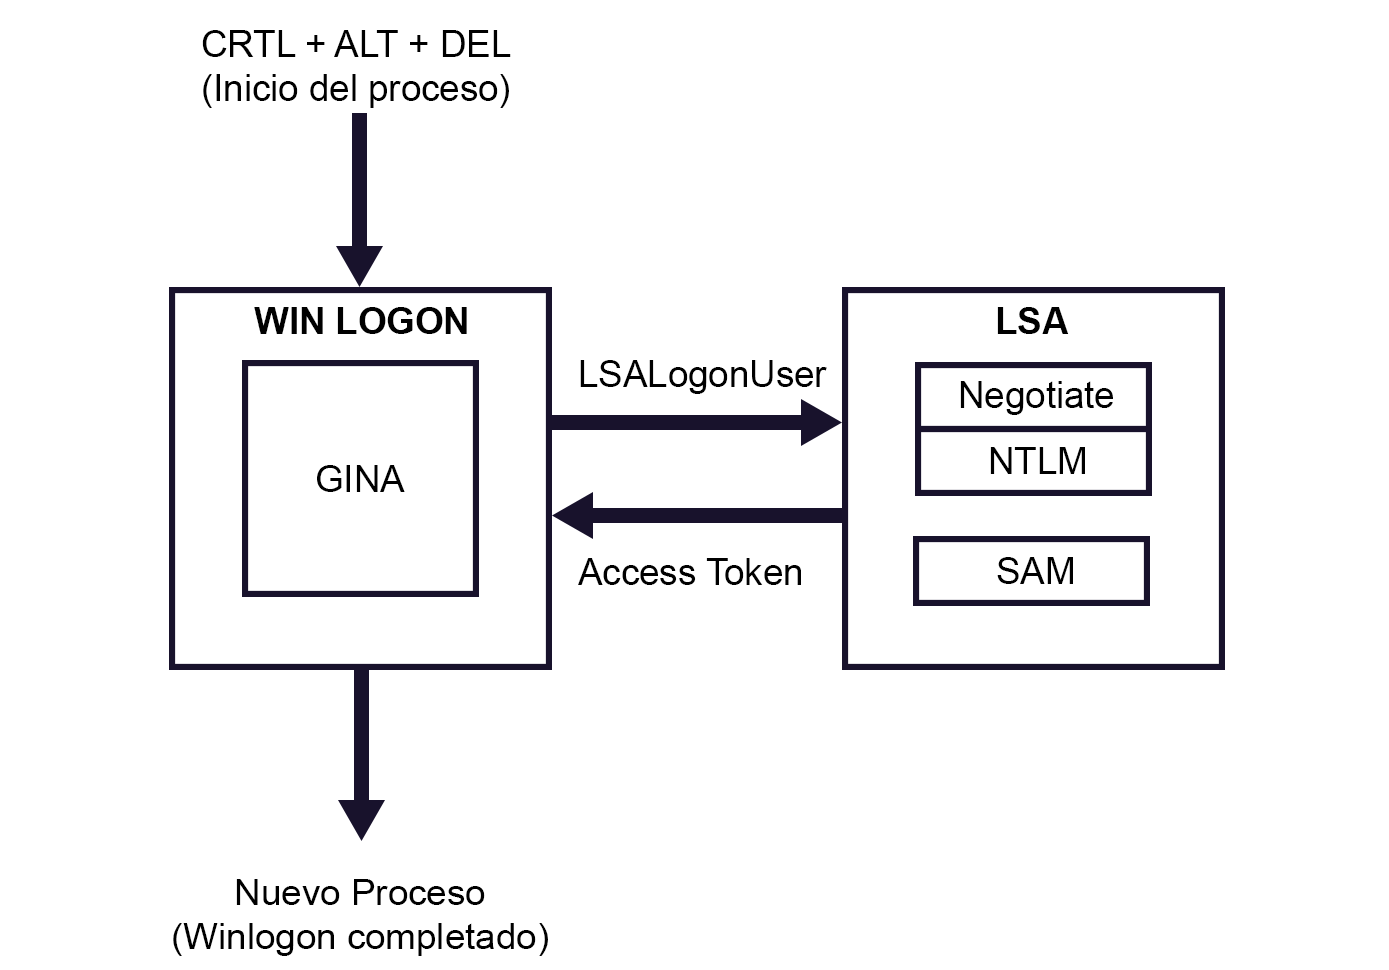
\includegraphics[width=16cm]{Local-Logon.png}
\end{center}
\caption{Fases de Inicio de Sesión Local (Local Logon)}
\label{local-logon}
\end{figure}
Como se puede observar en la figura \ref{local-logon} el proceso consta de varias fases:
\begin{enumerate}
\item En primer lugar, se proceso de Inicio de Sesión comienza con una {\it Secure Attention Sequence (SAS)}, esta secuencia es {\it CTRL + ALT + DEL} por defecto. 
\item Posteriormente, se iniciar el proceso interactivo, WinLogon se encarga de ello a través de tres partes: El propio ejecutable WinLogon, una biblioteca de enlace dinámico (DLL) encargada de la autenticación y la autorización gráfica llamada {\it Authentication dynamic-link library (GINA)} y cualquier proveedor de red.
\item El usuario introduce las credenciales pertinentes. GINA se encarga de recogerlas y llamar al proceso que se va a encargar de su validación: {\it Local Security Authority (LSA)}.
\item LSA verifica la identidad del usuario a través de las credenciales introducidas, si la validación se efectúa correctamente LSA devuelve al proceso WinLogon un Token de Acceso o {\it Access Token}. Para ello, en la fase de {\it Negotiate} se negocia el protocolo a usar, es decir, cómo se va a proceder la verificación, en este caso se utiliza NTLM. Las credenciales se validad contra la {\it Security Accounts Manager (SAM)} donde se encuentra las credenciales del usuario cifradas a través de NTLM y si estas son las mismas se procede a entregar el Token de Acceso.
\item Por último, WinLogon y GINA crean un nuevo proceso con dicho Token. 
\end{enumerate}

\subsubsection{Domain Logon}

\begin{figure}[t!] %[ht!] para here [b] para bottom [t] para top
\begin{center}
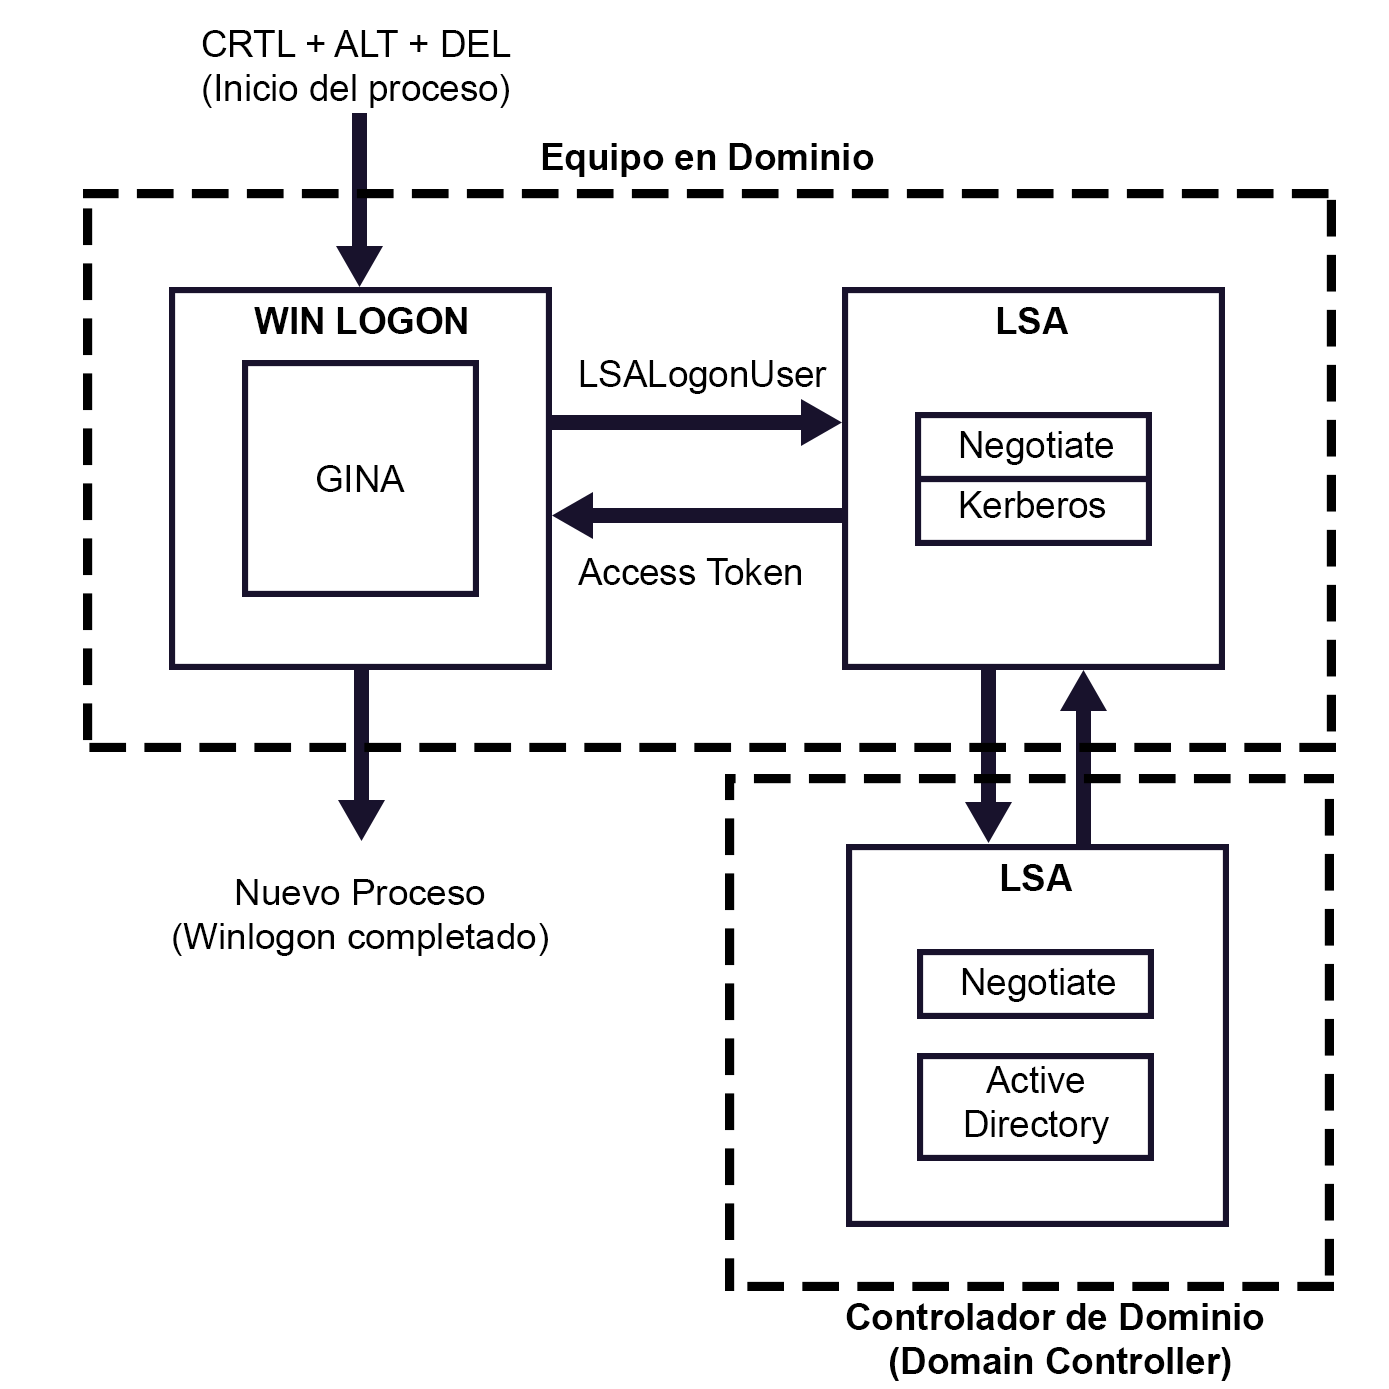
\includegraphics[width=16cm]{Domain-Logon.png}
\end{center}
\caption{Fases de Inicio de Sesión en Red (Domain Logon)}
\label{domain-logon}
\end{figure}
Como se puede observar en la Figura \ref{domain-logon} las fases implicadas en un inicio de sesión en red son muy similares las comentadas anteriormente en el proceso de Inicio de Sesión local, en este caso, el proceso {\it Local Security Authority (LSA)} determina si la validación es en local o a través del dominio. Posteriormente, otro proceso LSA ubicado en el dominio valida las credenciales introducidas por el usuario durante el Inicio de Sesión con los datos que hay en el dominio. Después de determinar cómo ha de ser esa validación (a través del protocolo NTLM o a través de Kerberos) los paquetes correspondientes validan al usuario.\\

\subsection{Authentication dynamic-link library (GINA)}

Como se ha comentado en el apartado anterior, {\it Authentication dynamic-link library (GINA)} es una Biblioteca de Enlace Dinámico, del inglés {\it Dynamic-Link Library (DLL)} 



\section{NT Lan Managey (NTLM) y Kerberos}

\section{Active Directory}

